\chapter{Performance Evaluation}\label{cha:performance-evaluation}

As \cite{guo2020ris}, we consider a RIS-aided femtocell network shown in Fig.\ref{fig:simulation_ris_setup}. The BS is equipped with a ULA array with $M=16$ antennas, and the RIS is equipped with
$N=20$ linearly-deployed reflecting elements. The system serves $K=4$ downlink users with a power budget of
$P=20$dBm and noise power of -117dBm. The direction of the radar target is $0^\circ$ from BS. 

\begin{figure}[htb]
  \centering
  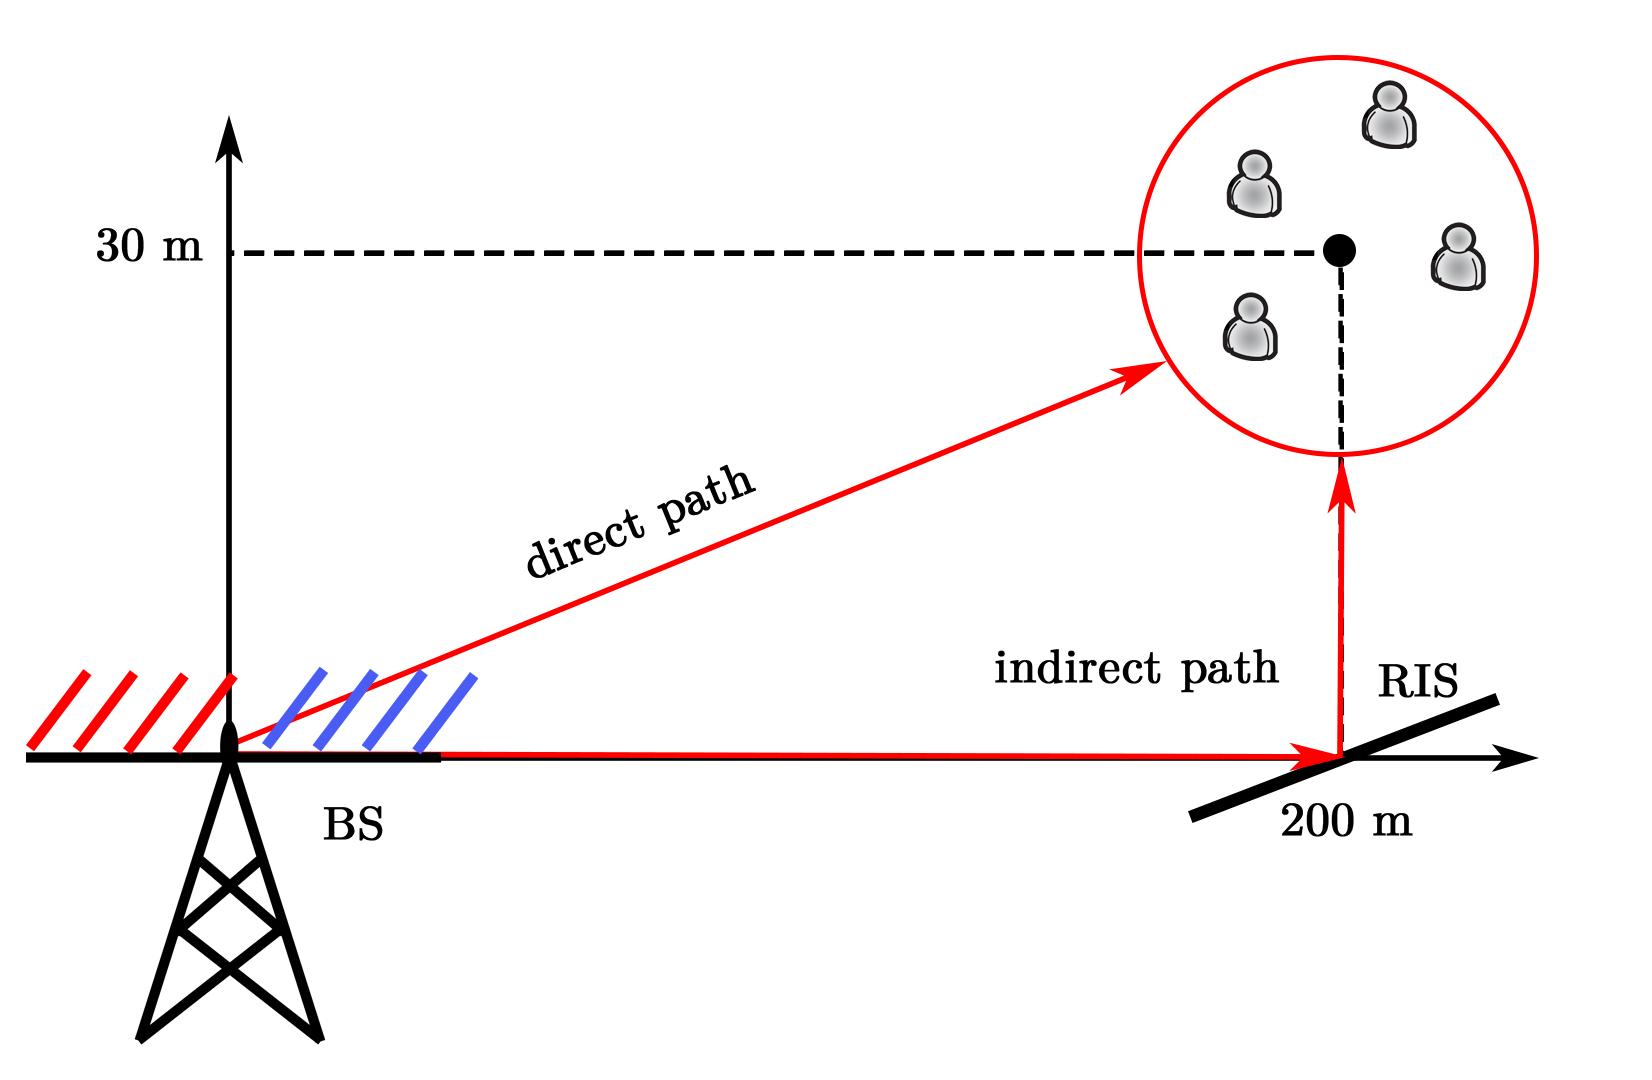
\includegraphics[width=0.8\textwidth]{simulation_ris_setup.png}
  \caption{The simulated RIS-aided femtocell network}
  \label{fig:simulation_ris_setup}
\end{figure}

In separated deployment, the resources are equally divided and allocated to radar and communication functions, 
i.e., $M_c=M_r=M/2$ and $P_c=P_r=P/2$. We assume that the BS-RIS and RIS-user channel 
follows the Rician fading and the BS-user channel experiences the Rayleigh fading. Thus, the channels
${\bf H}_c$, ${\bf H}_r$ and ${\bf h}_k$ are modeled as 
\begin{align}
    &{\bf H}_c = \sqrt{L_{BR}} \left( \sqrt{\frac{\varepsilon}{\varepsilon+1}} {\bf a}_{\mathrm{RIS}}(\vartheta) {\bf a}_c^H(\varphi) + \sqrt{\frac{1}{\varepsilon+1}} \check{\bf H}_c \right) \\
    &{\bf H}_r = \sqrt{L_{BR}} \left( \sqrt{\frac{\varepsilon}{\varepsilon+1}} {\bf a}_{\mathrm{RIS}}(\vartheta) {\bf a}_r^H(\varphi) + \sqrt{\frac{1}{\varepsilon+1}} \check{\bf H}_r \right) \\
    &{\bf h}_k = \sqrt{L_{RU}} \left( \sqrt{\frac{\varepsilon}{\varepsilon+1}} {\bf a}_{\mathrm{RIS}}(\varsigma_k) + \sqrt{\frac{1}{\varepsilon+1}} \check{\bf h}_k \right)
\end{align}
where $L_{BR}$ and $L_{RU}$ are the path loss, $\varepsilon$ is the Rician factor and $(\check{\bf H}_c, \check{\bf H}_r, \check{\bf h}_k)$
are NLOS components that follow Rayleigh fading. The BS-user channels ${\bf d}_{r,k}$ and ${\bf d}_{c,k}$ are assumed to 
follow Rayleigh fading. In the baseline, only the direct channels ${\bf d}_{r,k}$ and ${\bf d}_{c,k}$ are considered. 

In shared deployment, the channel ${\bf H}$ is similarly formulated as
\begin{equation}
    {\bf H} = \sqrt{L_{BR}} \left( \sqrt{\frac{\varepsilon}{\varepsilon+1}} {\bf a}_{\mathrm{RIS}}(\vartheta) {\bf a}^H(\varphi) + \sqrt{\frac{1}{\varepsilon+1}} \check{\bf H} \right)
\end{equation}

Table \ref{tab:reference_parameters} shows the detailed simulation parameters which is similar to \cite{guo2020ris}. 
In particular, the path loss model is defined based on 3GPP propagation environment \cite{3gpp.36.814}.

\begin{table}[h!]
  \caption{Simulation parameters}
  \centering
  \begin{tabular}{lll}
                                & Parameter                          & Value                                \\ \hline
  \multirow{9}{*}{Transceiver}  & BS Location                        & $(0\mathrm{m},0\mathrm{m})$          \\
                                & RIS Location                       & $(200\mathrm{m},0\mathrm{m})$        \\
                                & User Location                      & within $10\mathrm{m}$ from $(30\mathrm{m},200\mathrm{m})$ \\
                                & Target Direction                   & $0^\circ$ from BS                    \\
                                & Number of Users                    & $K = 4$                              \\
                                & Antennas at BS                     & $M = 16$                             \\
                                & Reflecting Elements                & $N = 20$                             \\
                                & Transmit power                     & $P = 20$dBm                         \\
                                & Noise power                        & $\sigma _n^2 =  - 117$dBm           \\ \hline
  \multirow{2}{*}{Channel}      
                                & Indirect Path Loss                 & $35.6+22.0 \log_{10}(d)$ dB          \\
                                & Direct Path Loss                   & $32.6+36.7 \log_{10}(d)$ dB
  \end{tabular}
  \label{tab:reference_parameters}
\end{table}

\section{Convergence}\label{sec:convergence}
  The convergence of the proposed algorithms is demonstrated in this part. Figure \ref{fig:convergence} shows that the proposed
algorithms for both separated and shared deployments can converge in 10 iterations, which indicates the low complexity of the 
proposed algorithms.
\newpage

\begin{figure}[ht]
    \centering
    \subfigure[Algorithm for separated deployment]{
        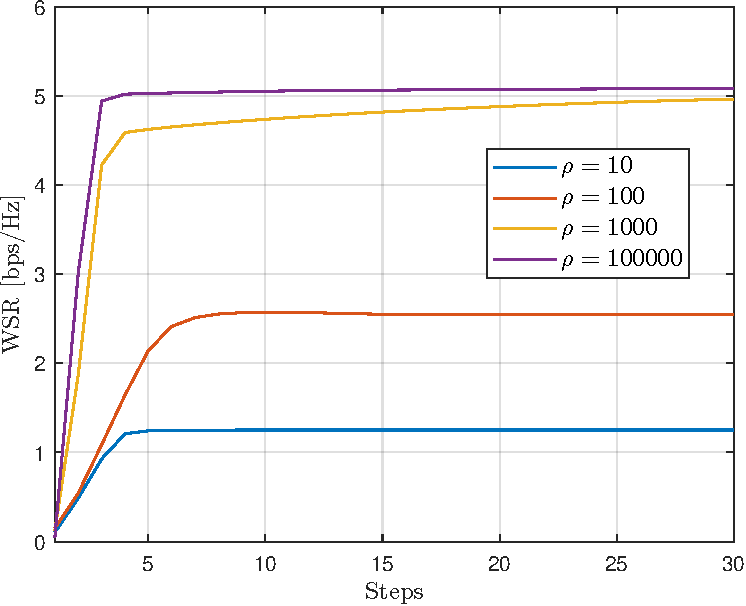
\includegraphics[width=0.475\textwidth]{convergence_separated.pdf}
        \label{fig:convergence_separated}
    }
    \subfigure[Algorithm for shared deployment]{
	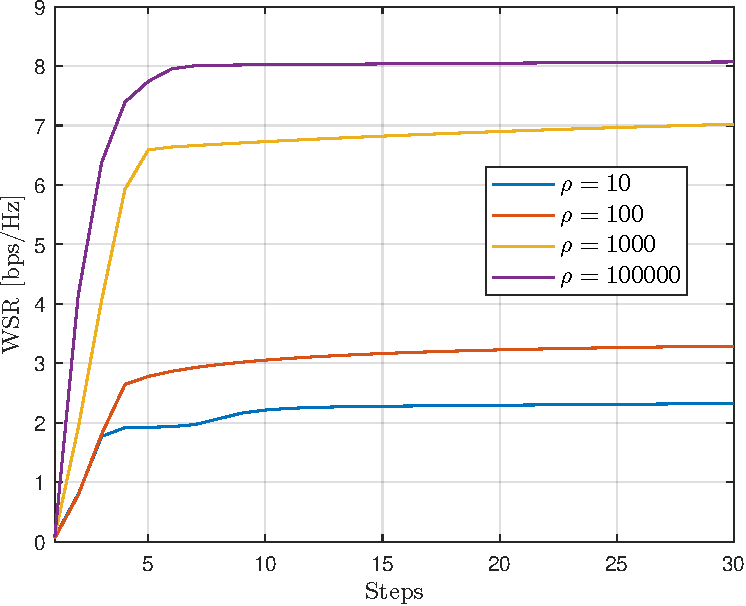
\includegraphics[width=0.475\textwidth]{convergence_shared.pdf}
        \label{fig:convergence_shared}
    }
    \caption{Convergence of proposed algorithms}
    \label{fig:convergence}
\end{figure}

Note that in Figure \ref{fig:convergence_shared}, the eigenvalue decomposition in used to approximate $\tilde{\bf p}_k^\star$ 
in SDR. In Figure \ref{fig:convergence_compare}, we compare the eigenvalue decomposition and Gaussian randomization in Algorithm \ref{alg:B}
when $\rho=100000$. It can be observed that the algorithm cannot converge when the Gaussian randomization is applied. 
The reason is that the $\tilde{\bf T}_k^\star$ calculated by CVX toolbox in practice is almost rank-one, i.e., the eigenvalues except
the largest one are almost zero. In this case, the Gaussian randomization cannot guarantee a good rank-one approximation.

\begin{figure}[ht]
    \centering
    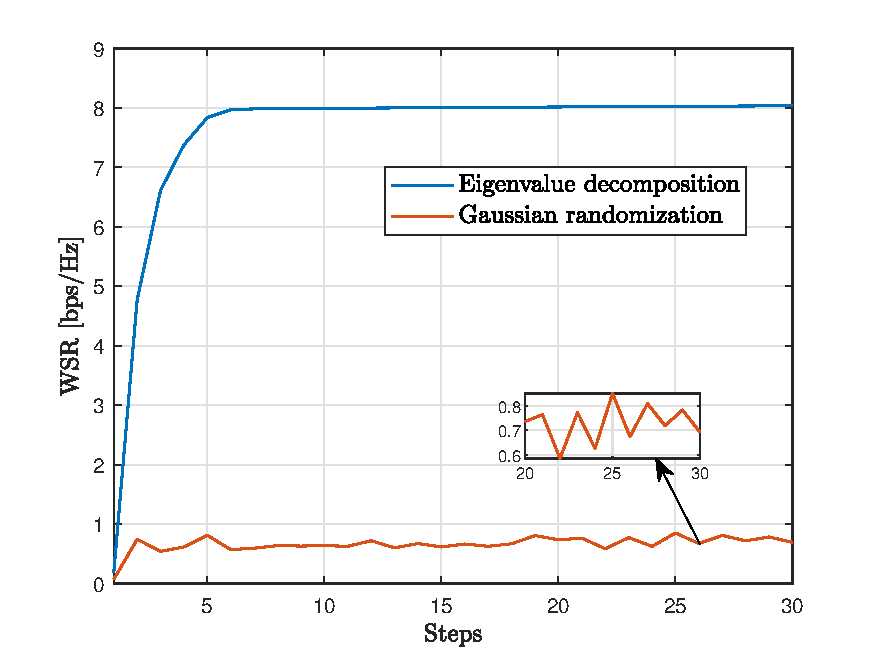
\includegraphics[width=0.6\textwidth]{convergence_shared_compare.pdf}
    \caption{Comparison of eigenvalue decomposition and Gaussian randomization}
    \label{fig:convergence_compare}
\end{figure}

\section{Transmission Beampattern Comparison}\label{sec:beampattern_compare}
  In this section, we demonstrate the beampatterns obtained from Algorithm \ref{alg:A} and \ref{alg:B} 
and the baselines in both LOS-dominated Rician channel and Rayleigh channel.

Figure \ref{fig:beampattern_rayleigh_single_fully} compares the averaged beampattern from Monte-Carlo simulation when BS-RIS and RIS-user channels follow 
Rayleigh fading ($\varepsilon = 0$).
One can visualize from Figure \ref{fig:beampattern_rayleigh_single_fully_a} and \ref{fig:beampattern_rayleigh_single_fully_c} that both single connected and fully connected RIS make tiny improvement to the beampattern 
compared with baseline when the WSR is small. However, as shown in Figure \ref{fig:beampattern_rayleigh_single_fully_b} and \ref{fig:beampattern_rayleigh_single_fully_d}, when WSR increases to a large value, i.e., $5.4$bps/Hz and $7.9$bps/Hz, fully connected 
RIS achieves the largest probing power at target. The gains achieved by fully connected RIS in separated deployment 
over single connected RIS and baseline are 2.2dB and 4.7dB, respectively. The counterparts in shared deployment are 2.7dB and 4.8dB.

\begin{figure}[ht]
    \centering
    \subfigure[Separated deployment: WSR = $1.0$bps/Hz]{
        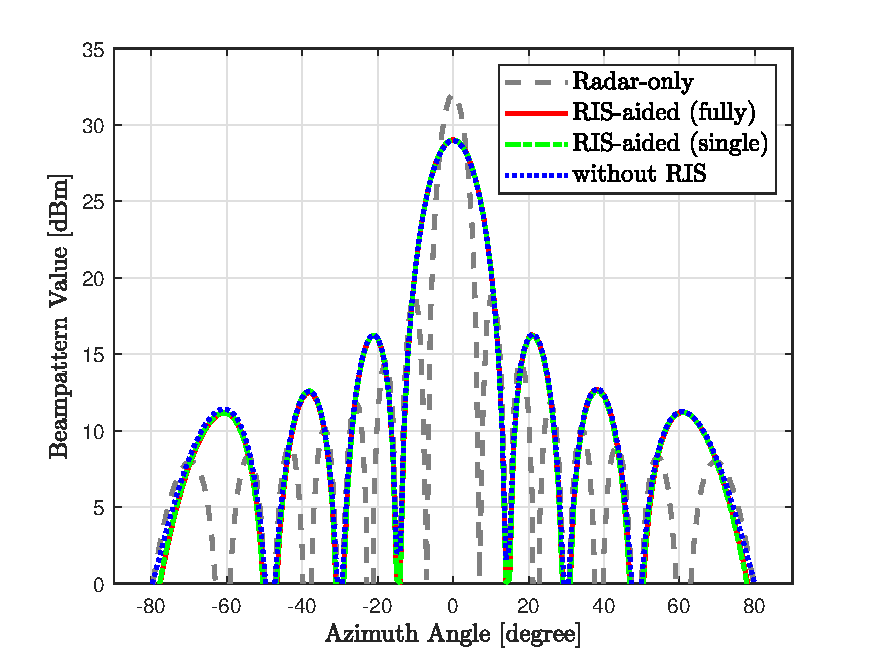
\includegraphics[width=0.475\textwidth]{beampattern_rayleigh_single_fully_a.pdf}
        \label{fig:beampattern_rayleigh_single_fully_a}
    }
    \subfigure[Separated deployment: WSR = $5.4$bps/Hz]{
	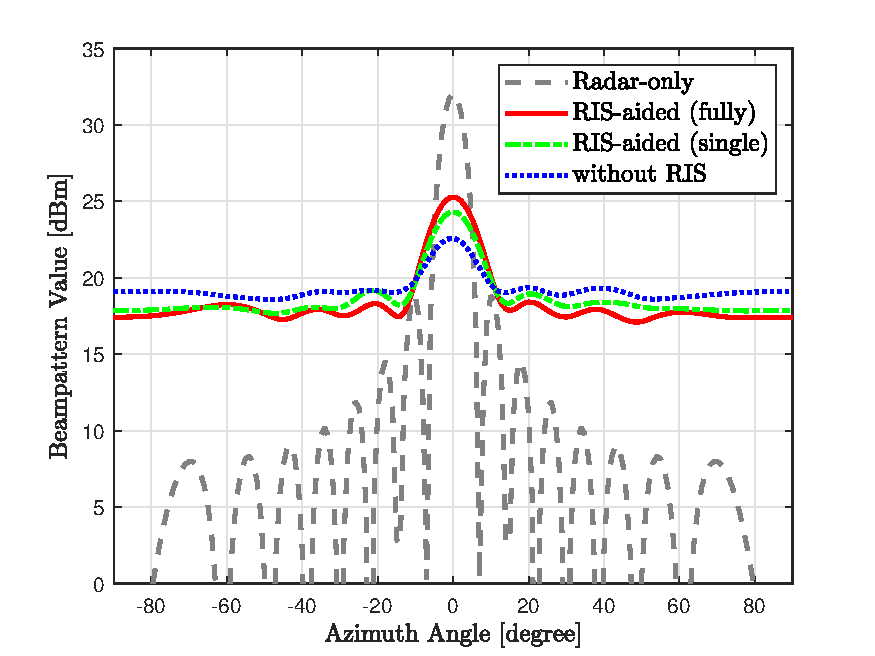
\includegraphics[width=0.475\textwidth]{beampattern_rayleigh_single_fully_b.pdf}
        \label{fig:beampattern_rayleigh_single_fully_b}
    }

    \subfigure[Shared deployment: WSR = $1.8$bps/Hz]{
        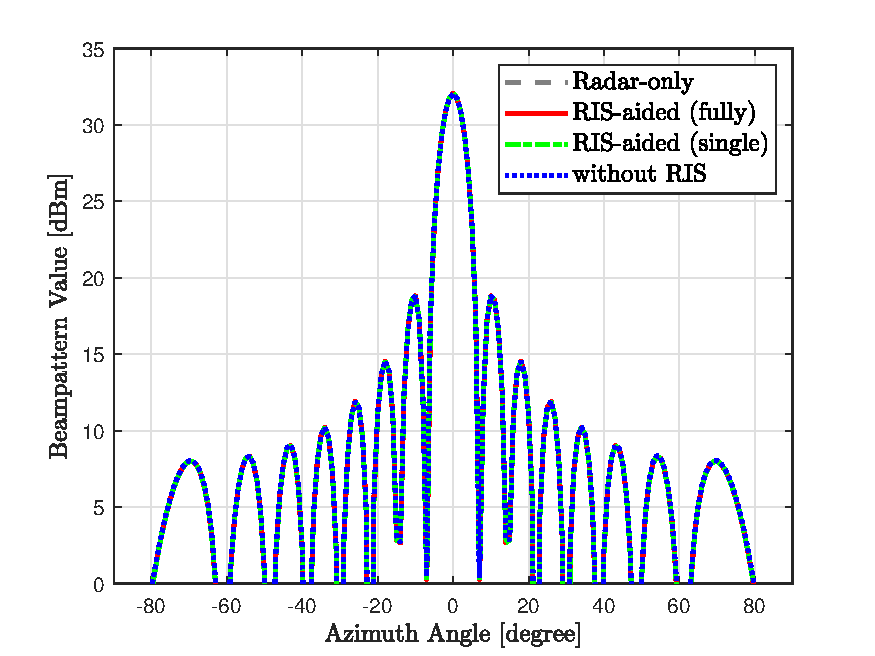
\includegraphics[width=0.475\textwidth]{beampattern_rayleigh_single_fully_c.pdf}
        \label{fig:beampattern_rayleigh_single_fully_c}
    }
    \subfigure[Shared deployment: WSR = $7.9$bps/Hz]{
	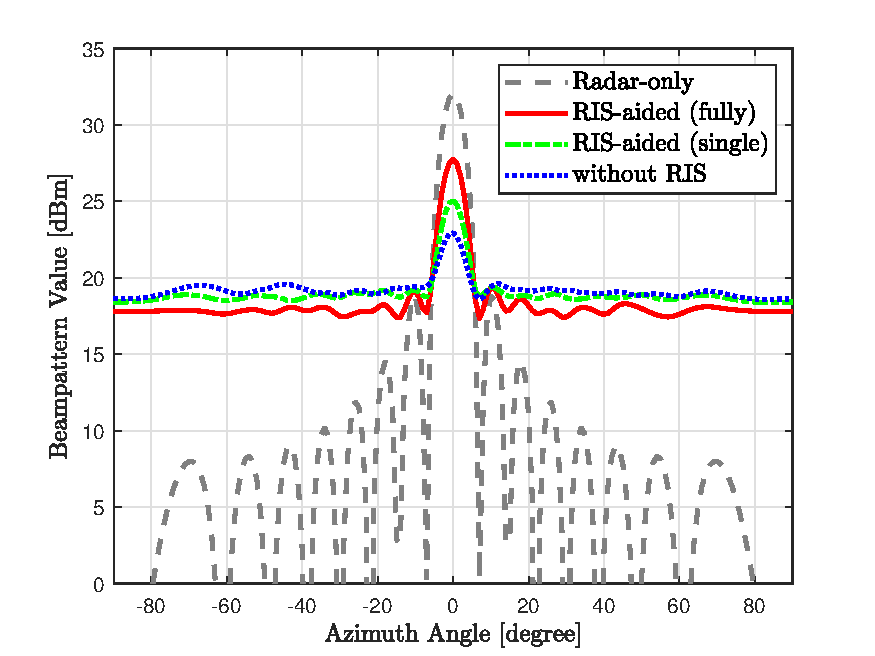
\includegraphics[width=0.475\textwidth]{beampattern_rayleigh_single_fully_d.pdf}
        \label{fig:beampattern_rayleigh_single_fully_d}
    }
    \caption{Beampattern comparison in Rayleigh channel ($\varepsilon = 0$)}
    \label{fig:beampattern_rayleigh_single_fully}
\end{figure}

Figure \ref{fig:beampattern_los_single_fully} compares the averaged beampattern when the BS-RIS and RIS-user channels are LOS-dominated  Rician channel ($\varepsilon = 1000$). 
We can see that in both separated and shared deployment the fully connected RIS does not outperform the single connected RIS significantly in terms of probing power no matter the 
WSR is large or small. Therefore, the fully connected only shows advantages when the BS-RIS and RIS-user channels follow Rayleigh fading.
The scaling law in \cite{shen2020modeling} indicates that the fully connected and single connected RIS achieves the same 
received power at users in LOS channel because the model of LOS channel leads to the same optimal ${\bf \Theta}$. This scaling law
can also explain the results in Figure \ref{fig:beampattern_los_single_fully}: the model of LOS channel also leads to the same optimal ${\bf \Theta}$ in terms of WSR, 
so that the WSR is the same when the probing power at target is the same. 

\begin{figure}[ht]
    \centering
    \subfigure[Separated deployment: WSR = $1.0$bps/Hz]{
        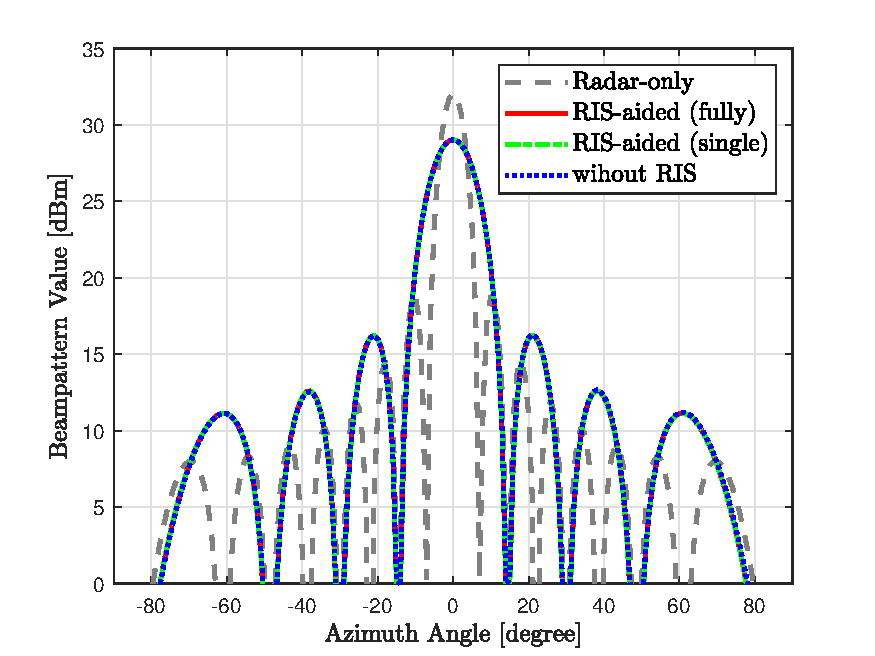
\includegraphics[width=0.475\textwidth]{beampattern_los_single_fully_a.pdf}
        \label{fig:beampattern_los_single_fully_a}
    }
    \subfigure[Separated deployment: WSR = $5.4$bps/Hz]{
    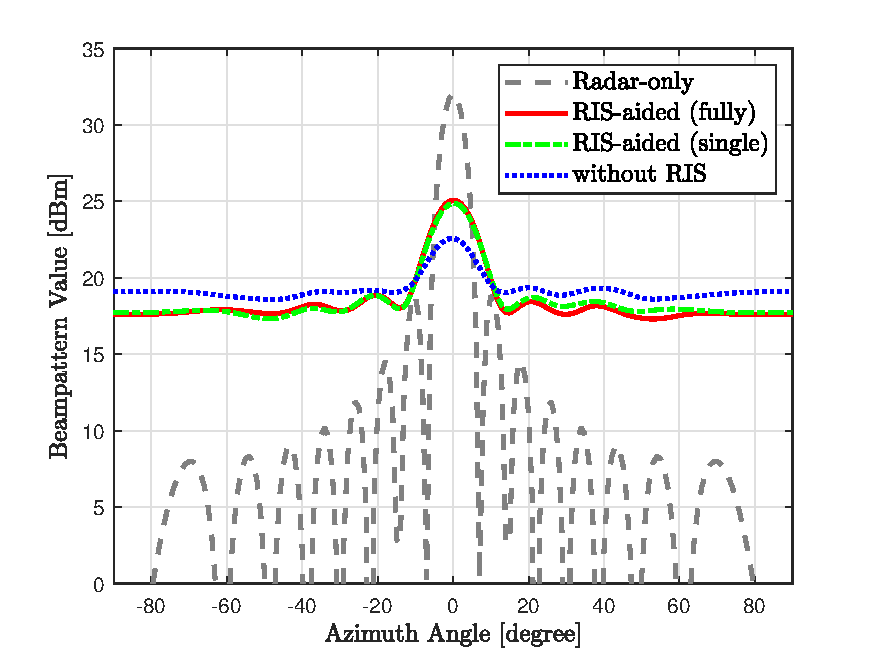
\includegraphics[width=0.475\textwidth]{beampattern_los_single_fully_b.pdf}
        \label{fig:beampattern_los_single_fully_b}
    }

    \subfigure[Shared deployment: WSR = $1.8$bps/Hz]{
        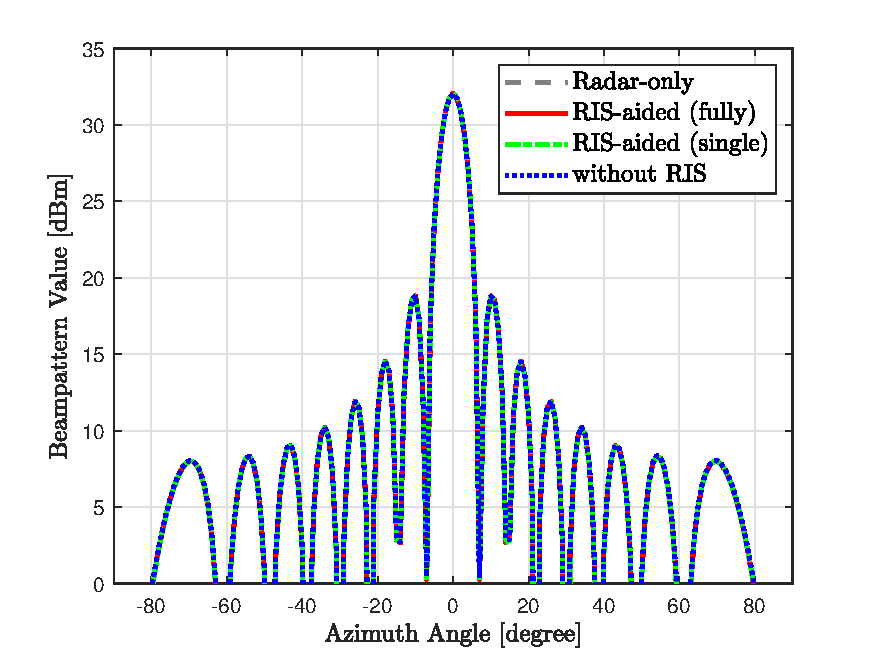
\includegraphics[width=0.475\textwidth]{beampattern_los_single_fully_c.pdf}
        \label{fig:beampattern_los_single_fully_c}
    }
    \subfigure[Shared deployment: WSR = $7.9$bps/Hz]{
    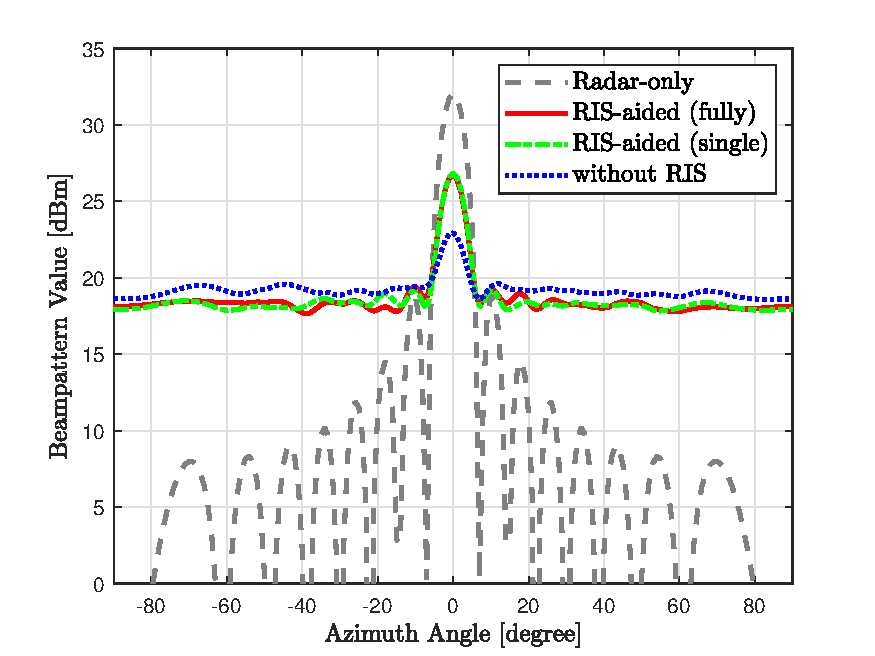
\includegraphics[width=0.475\textwidth]{beampattern_los_single_fully_d.pdf}
        \label{fig:beampattern_los_single_fully_d}
    }
    \caption{Beampattern comparison in LOS-dominated  Rician channel ($\varepsilon = 1000$)}
    \label{fig:beampattern_los_single_fully}
\end{figure}



Figure \ref{fig:beampattern_reflecting_elements} shows the effect of the number of reflecting elements in LOS-dominated  Rician channel. As the fully connected and 
single connected RIS perform the same in LOS channel, only single connected RIS is considered in Figure \ref{fig:beampattern_reflecting_elements}. We can see that 
the better beampattern and higher probing power at target are achieved as the growth of element amounts. Nevertheless, the improvement
is not to infinity but asymptotically reaches an upper bound. For example, in shared deployment, the probing power at target increases by
4.9dB as the reflecting element increases from 0 to 20, while the gains are reduced to 1.2dB and 0.2dB when the amount changes from 20 to 60 and from 60 to 100,
respectively.

Figure \ref{fig:beampattern_rayleigh_separated_shared} compares the beampattern of separated and shared deployments. It displays that the mainlobe of beampattern
in shared deployment is much more narrow than that in separated deployment, which is more directional. With the help of RIS,
the probing power at target in shared deployment is only $0.13$dB lower than the Radar-only system when there are 100 reflecting elements.

\begin{figure}
	\centering
	\begin{minipage}[t]{1\linewidth}
        \centering
        \subfigure[Separated deployment: WSR = $5.4$bps/Hz]{
        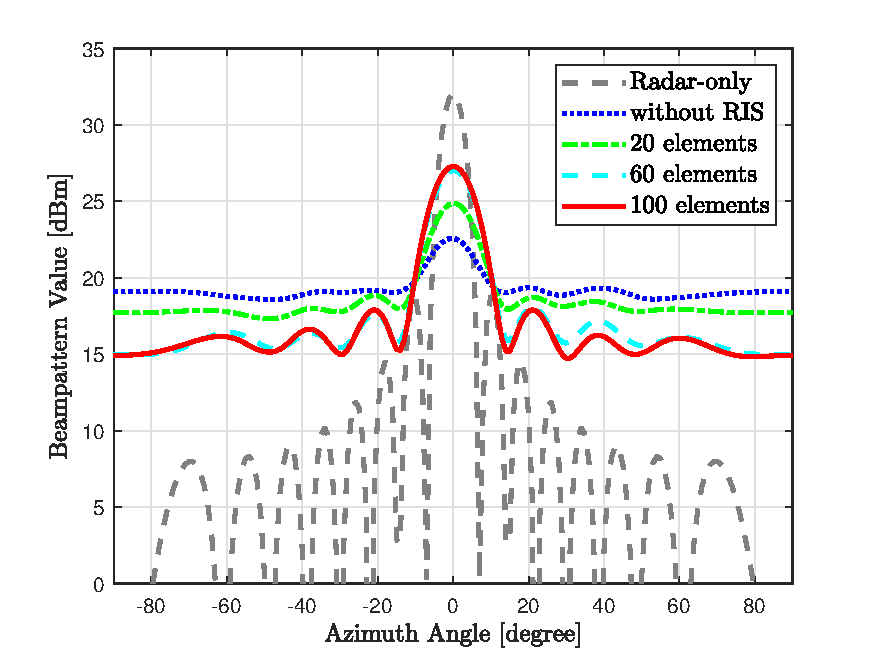
\includegraphics[width=0.475\textwidth]{beampattern_reflecting_elements_a.pdf}
            \label{fig:beampattern_reflecting_elements_a}
        }
        \subfigure[Shared deployment: WSR = $7.9$bps/Hz]{
        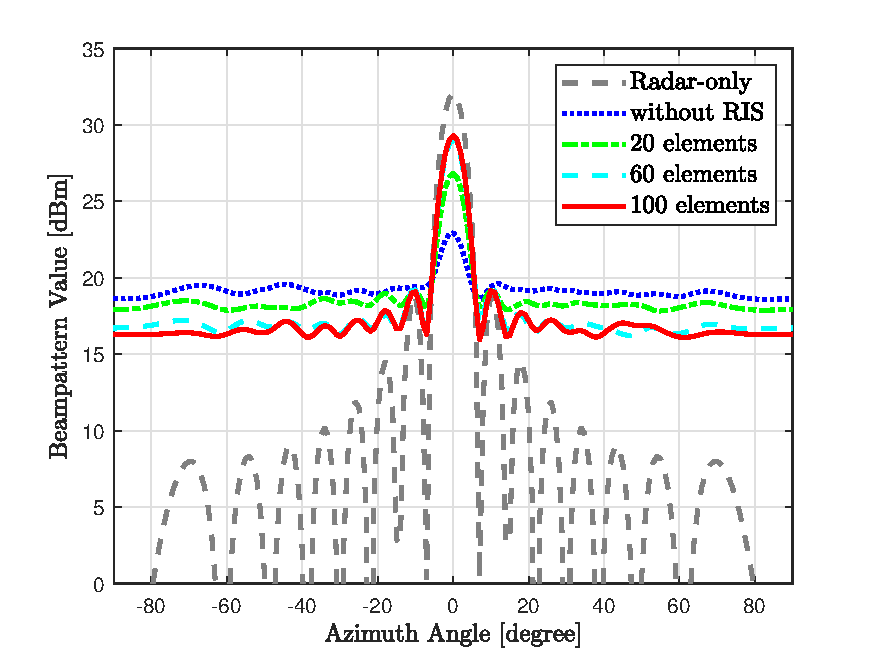
\includegraphics[width=0.475\textwidth]{beampattern_reflecting_elements_b.pdf}
            \label{fig:beampattern_reflecting_elements_b}
        }
        \caption{Effect of the number of reflecting elements on beampattern in LOS-dominated Rician channel}
        \label{fig:beampattern_reflecting_elements}
	\end{minipage}
	\\
	\begin{minipage}[t]{1\linewidth}
        \centering
        \subfigure[without RIS, WSR = $5.4$bps/Hz]{
            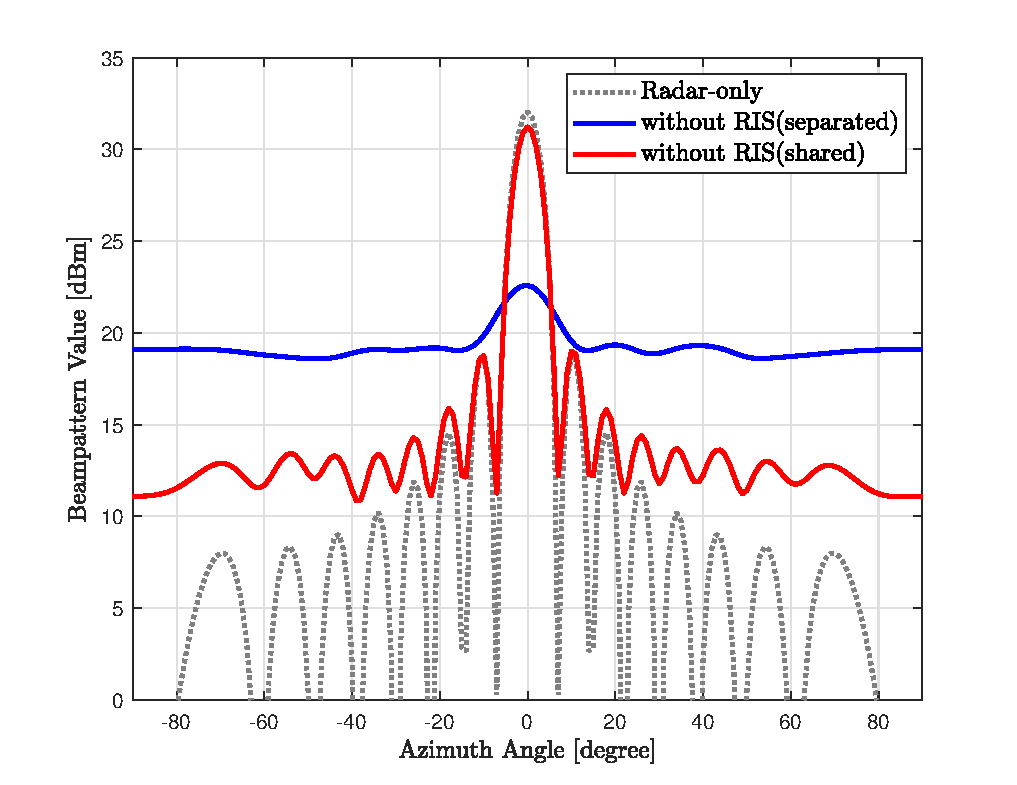
\includegraphics[width=0.475\textwidth]{beampattern_rayleigh_separated_shared_a.pdf}
            \label{fig:beampattern_rayleigh_separated_shared_a}
        }
        \subfigure[20 elements, WSR = $5.4$bps/Hz]{
        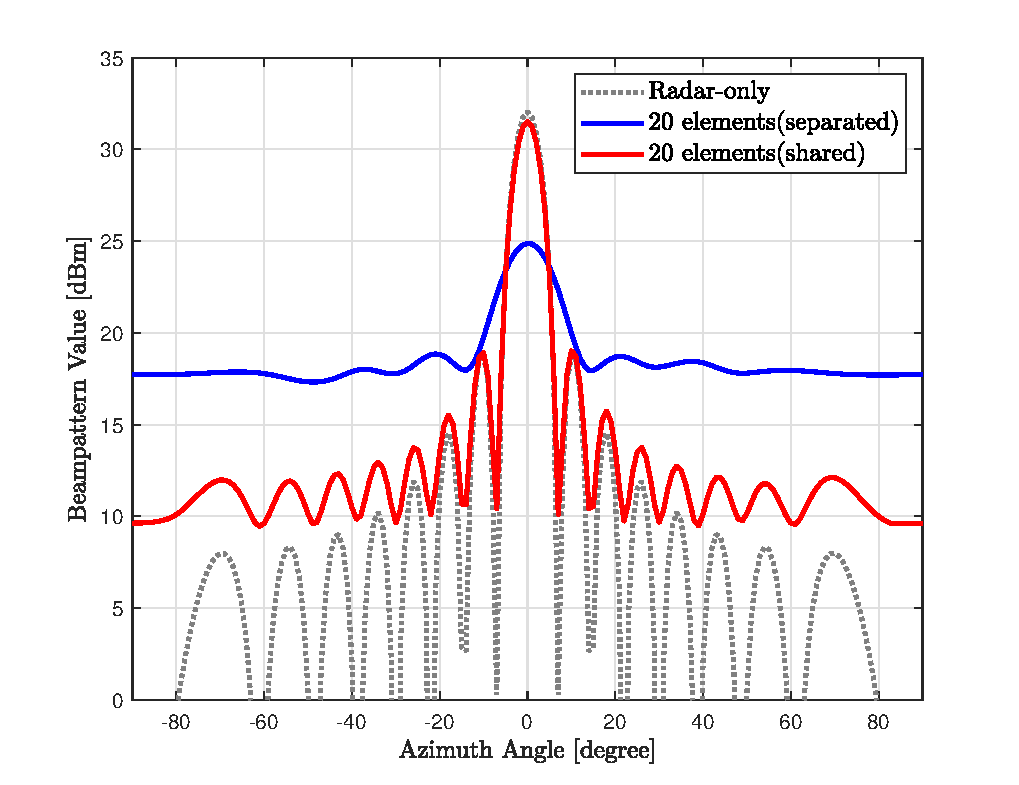
\includegraphics[width=0.475\textwidth]{beampattern_rayleigh_separated_shared_b.pdf}
            \label{fig:beampattern_rayleigh_separated_shared_b}
        }
    
        \subfigure[60 elements, WSR = $5.4$bps/Hz]{
            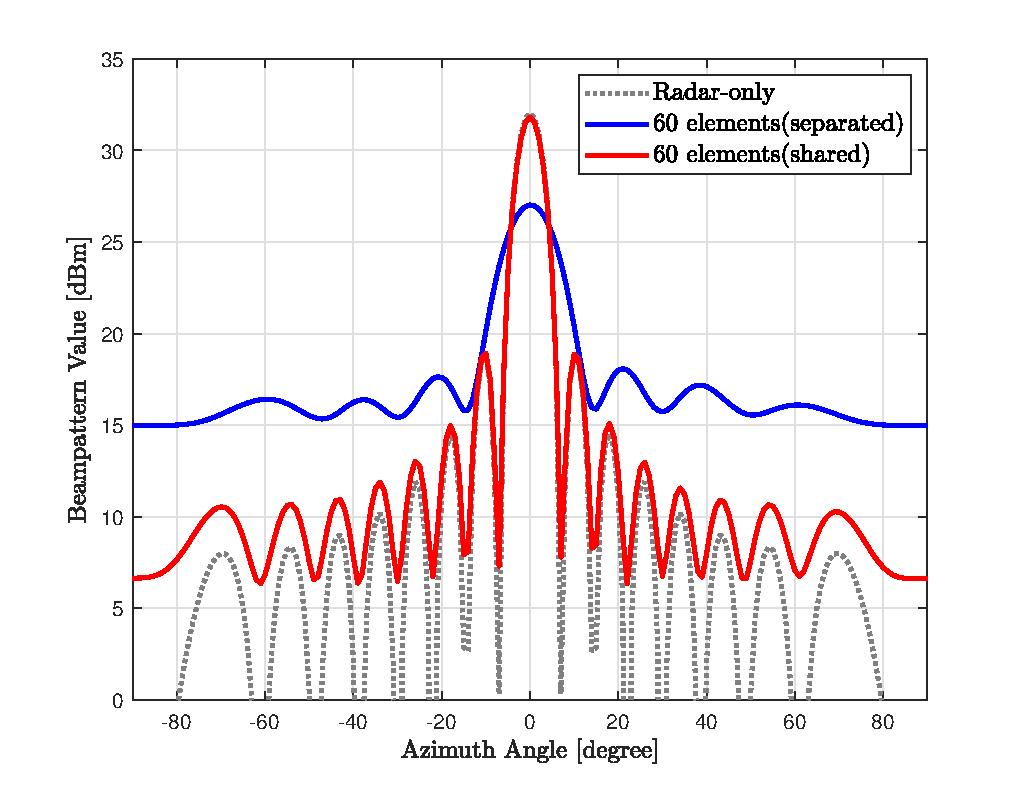
\includegraphics[width=0.475\textwidth]{beampattern_rayleigh_separated_shared_c.pdf}
            \label{fig:beampattern_rayleigh_separated_shared_c}
        }
        \subfigure[100 elements, WSR = $5.4$bps/Hz]{
        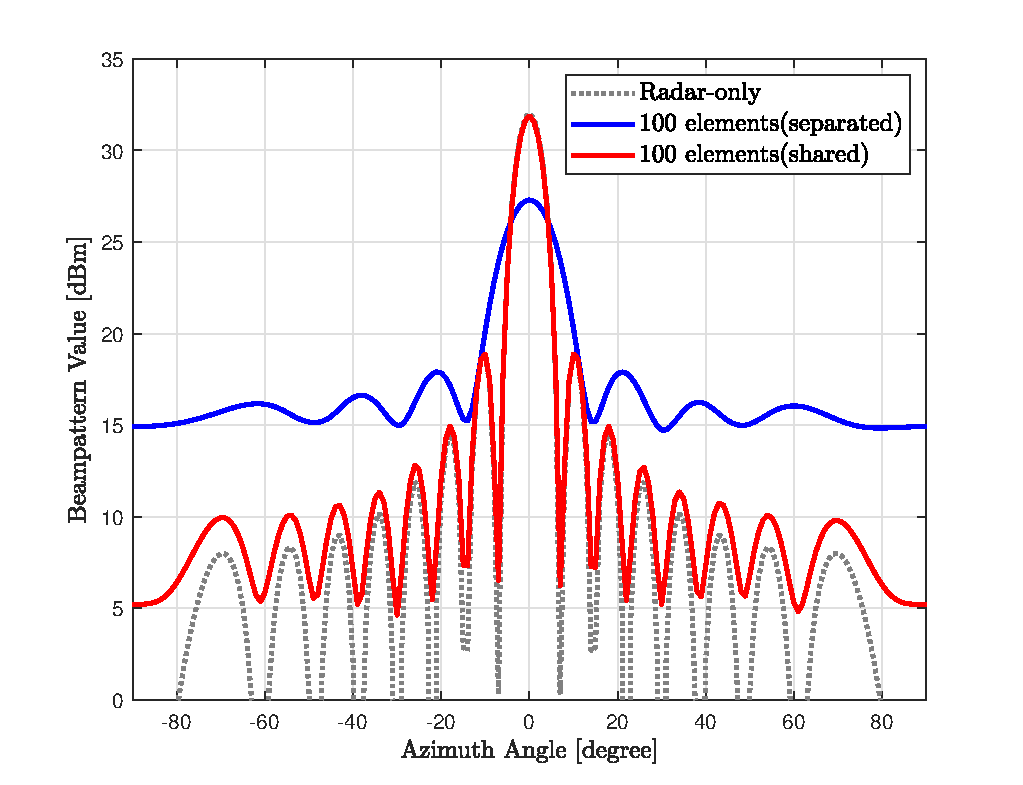
\includegraphics[width=0.475\textwidth]{beampattern_rayleigh_separated_shared_d.pdf}
            \label{fig:beampattern_rayleigh_separated_shared_d}
        }
        \caption{Beampattern comparison of separated and share deployment in LOS-dominated Rician channel}
        \label{fig:beampattern_rayleigh_separated_shared}
	\end{minipage}
\end{figure}
\newpage

\section{Tradeoff Comparison}\label{sec:tradeoff_compare}
  As problem \eqref{problem:seperated_problem} and \eqref{problem:shared_problem} are multi-objective optimization problems, we can obtain
the Pareto optimal front by varying the regularization parameter $\rho$, which is
capable of revealing the tradeoff relationship between different objectives, i.e., 
probing power at target and WSR. Figure \ref{fig:tradeoff_single_fully} shows the Pareto optimal fronts 
of the RIS-aided and normal DFRC systems.

\begin{figure}[h]
    \centering
    \subfigure[Separated deployment: $\varepsilon = 0$]{
        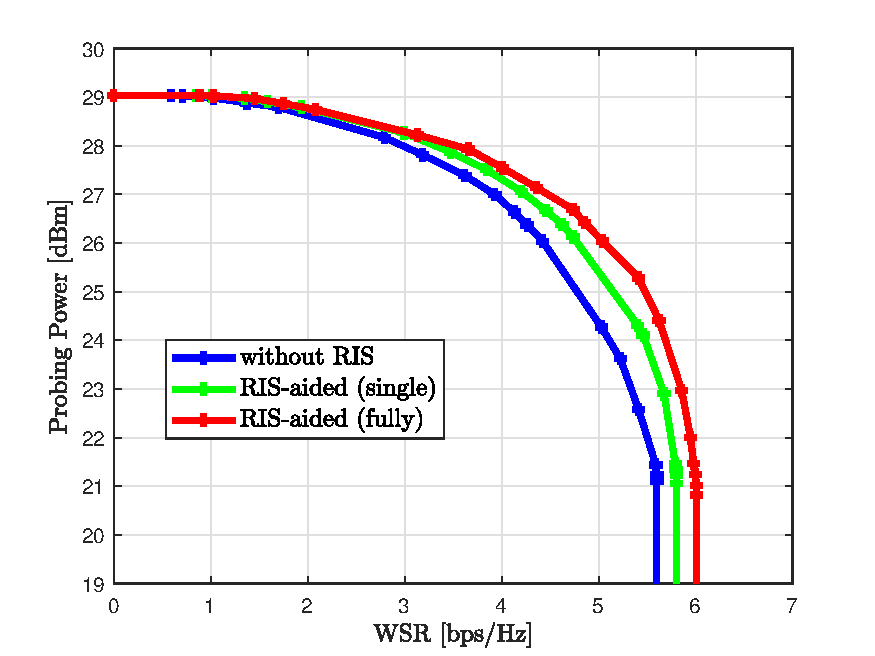
\includegraphics[width=0.475\textwidth]{tradeoff_single_fully_a.pdf}
        \label{fig:tradeoff_single_fully_a}
    }
    \subfigure[Separated deployment: $\varepsilon = 1000$]{
    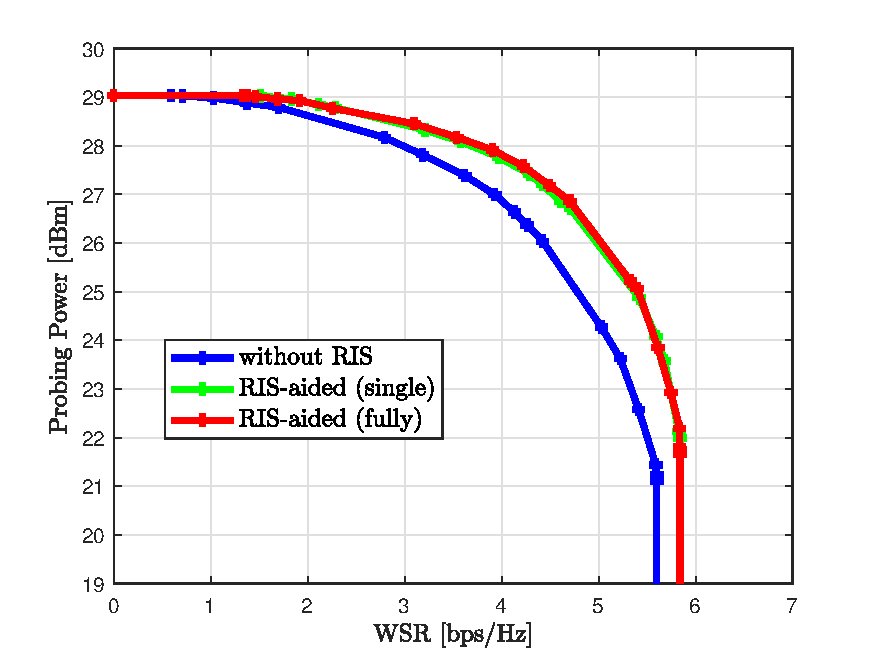
\includegraphics[width=0.475\textwidth]{tradeoff_single_fully_b.pdf}
        \label{fig:tradeoff_single_fully_b}
    }
    \subfigure[Shared deployment: $\varepsilon = 0$]{
        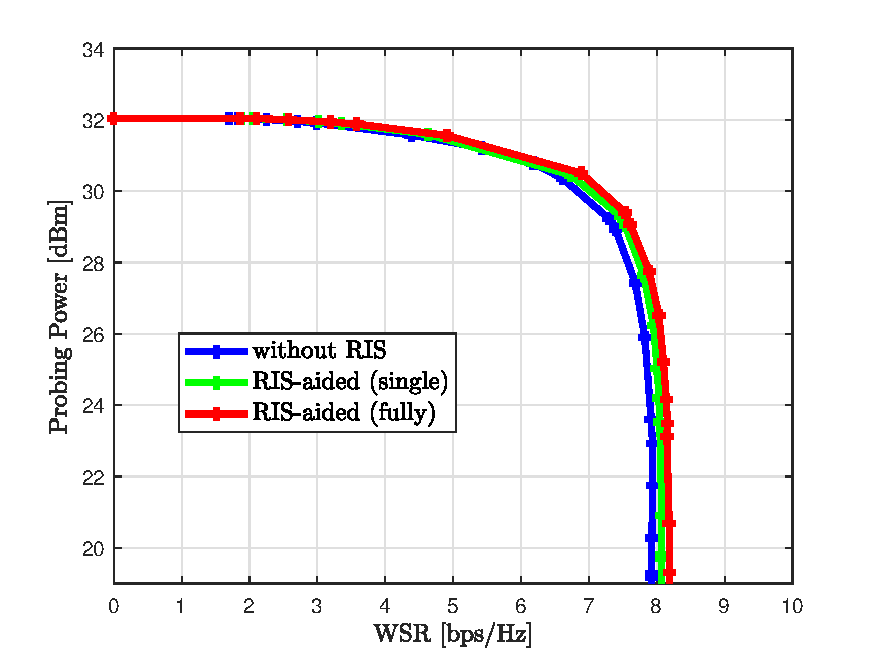
\includegraphics[width=0.475\textwidth]{tradeoff_single_fully_c.pdf}
        \label{fig:tradeoff_single_fully_c}
    }
    \subfigure[Shared deployment: $\varepsilon = 1000$]{
    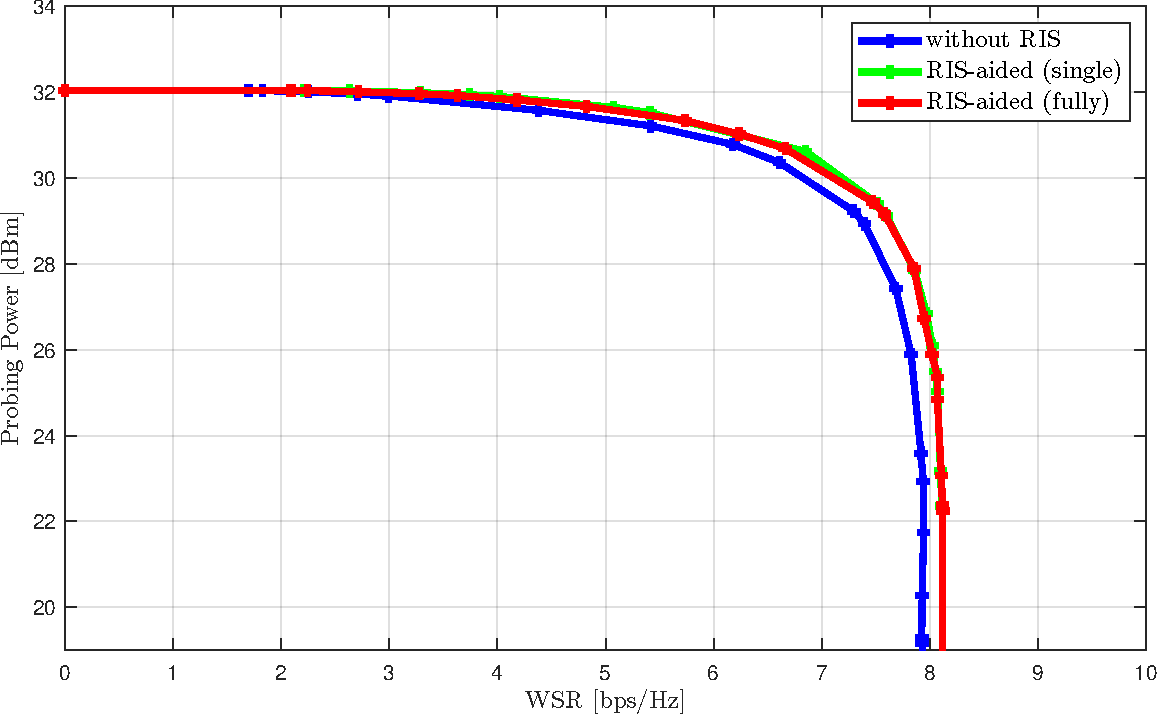
\includegraphics[width=0.475\textwidth]{tradeoff_single_fully_d.pdf}
        \label{fig:tradeoff_single_fully_d}
    }
    \caption{Tradeoff between probing power at target and WSR}
    \label{fig:tradeoff_single_fully}
\end{figure}

In Figure \ref{fig:tradeoff_single_fully_a}, it is obvious that we must decrease the probing power to increase 
the WSR and vice versa, which is a tradeoff. It is also clear that the RIS shows advantages 
compared with DFRC without RIS. 

For separated deployment, when the BS-RIS and RIS-user channels are Rayleigh channel (shown in Figure \ref{fig:tradeoff_single_fully_a}), 
the fully connected RIS performs best, which has a $6.0$bps/Hz upper bound of WSR. The single connected RIS is capable of 
achieving $5.8$bps/Hz upper bound of WSR, which is $0.20$bps/Hz higher than that achieved in the baseline. Figure \ref{fig:tradeoff_single_fully_b} 
shows that case where the channel is LOS dominated. One can visualize that the fully connected and single connected RIS has the same 
performance, which further validates the result in Section \ref{sec:beampattern_compare}.

Figure \ref{fig:tradeoff_single_fully_c} and \ref{fig:tradeoff_single_fully_d} show that the fully connected RIS only outperforms single connected RIS in Rayleigh channel for 
shared deployment, which is the same as separated deployment. However, the gain from RIS is smaller than that in separated deployment,
which is $0.15$bps/Hz and $0.27$bps/Hz for single connected and fully connected RIS in Rayleigh channel, respectively.

Although the RIS can increase the WSR upper bound, the 
probing power upper bounds are all $29$dBm in separated deployment and $32$dBm in shared deployment. 
The reason is that the probing power upper bound is determined by the capability of BS, which is the same when there is RIS or not.
There is a $3$dB gain of probing power upper bound for shared deployment over separated deployment.

We now evaluate the performance of DFRC aided by single connected RIS in LOS-dominated Rician channel with various numbers of reflecting elements. In Figure \ref{fig:tradeoff_reflecting_element}, we can see 
that the DFRC systems have the larger achievable region and higher WSR upper bounds as the increase of reflecting elements. The RIS 
with 100 elements is capable of improving the WSR by $0.82$bps/Hz in separated deployment and $0.58$bps/Hz in shared deployment. 
\begin{figure}[h]
    \centering
    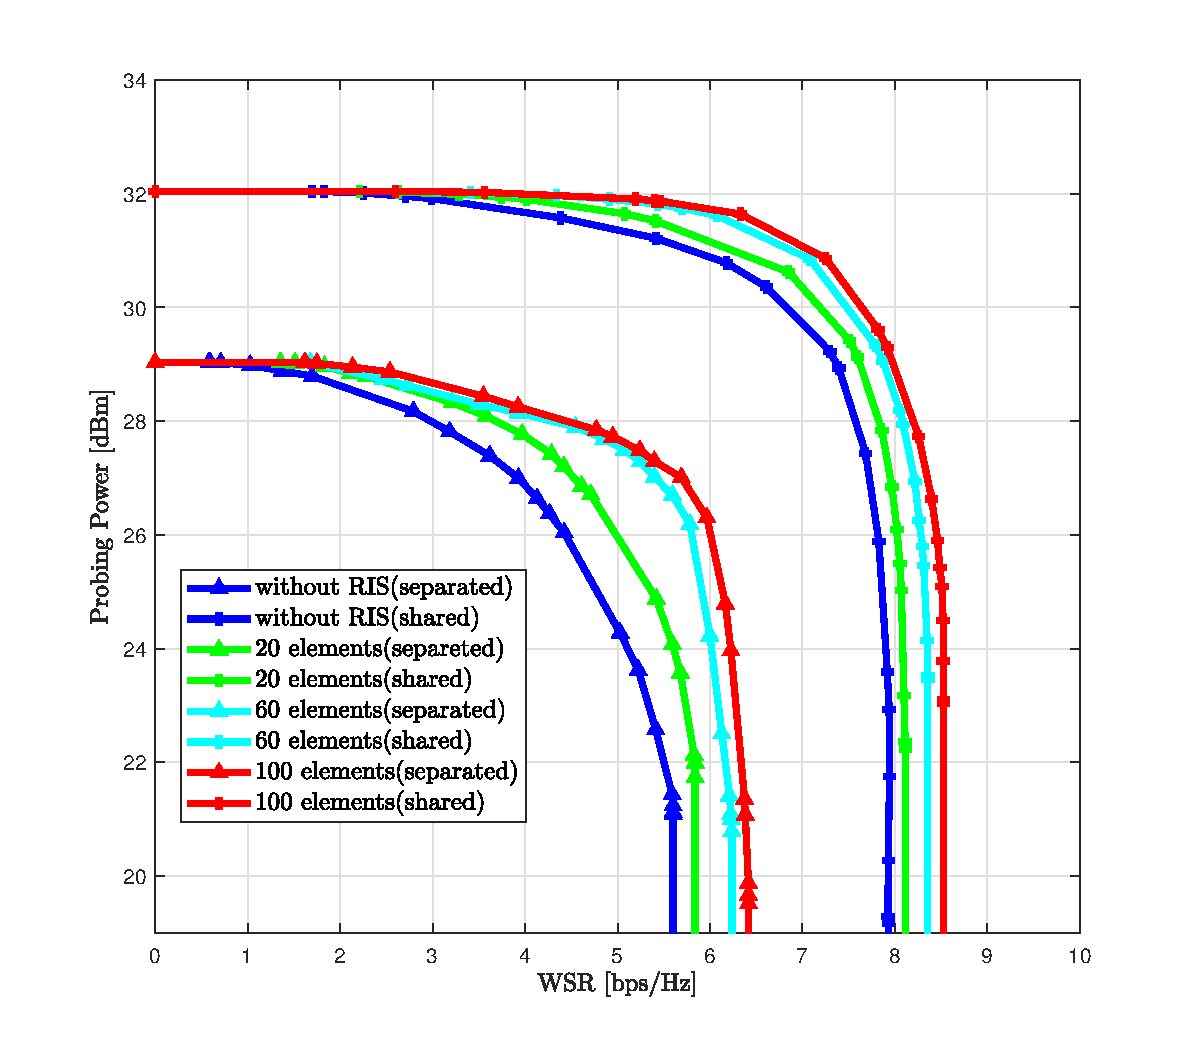
\includegraphics[width=1.0\textwidth]{tradeoff_reflecting_element.pdf}
    \caption{Effect of the number of reflecting elements on tradeoff in Rayleigh channels}
    \label{fig:tradeoff_reflecting_element}
\end{figure}


% \section{MIMO}\label{sec:mimo}
%   \input{performance-evaluation/mimo.tex} 